


\hypertarget{SSCmain}{}\section{SSC -\/ Source Spectrum Calculation}\label{SSCmain}
\begin{DoxyVersion}{Version}
x 
\end{DoxyVersion}
\begin{DoxyAuthor}{Author}
Markus Hoetzel (\href{mailto:markus.hoetzel@kit.edu}{\tt markus.hoetzel@kit.edu}) 
\end{DoxyAuthor}
\begin{DoxyDate}{Date}
2010
\end{DoxyDate}
\begin{DoxyAttention}{Attention}
The source of this documentation can be found in: /Modules/SSC/include/SSCToolBox.h. Some links in the Userguide will not work, since there targets are only contained in the Referenceguide.

\end{DoxyAttention}

\subsection{Introduction}\label{_s_s_cmain_Introduction}
The parameters of the source have to be known precisely because they are a main systematic uncertainty for the whole measurement of the neutrino mass:

A detailed model of the source is required to investigate the influence of various source parameters. The task of the package \char`\"{}Source Spectrum Calculations\char`\"{} SSC was to combine existing models to one central source model and to implement further models. Former calculations and source models considered the WGTS as a 10 m tube at whole and were not able to account for spatial variations of several source parameters that definitely occur. Dividing the source into small pieces, what is implemented in the developed program code SSC, allows for a very detailed investigation of the influence of source parameters on the integrated beta spectrum. These integrated spectra are calculated for every part of the WGTS using the local physical parameters. A combination of the spectra from all parts of the source gives the spectrum of the whole source, that can be investigated. It is now possible to study the effects of many different source parameters on the integrated beta spectrum of KATRIN. It should be emphasized here that calculations based on distribution functions of the source parameters were performed instead of single particle simulations. The task of SSC in the frame of Kassiopeia is to provide a realistic source model for the particle generators of KPAGE to simulate electrons from the source through the spectrometers to the detector using one program: Kassiopeia.
\subsection{General: WGTS}\label{_s_s_cmain_summaryWGTS}
The Windowless Gaseous Tritium Source WGTS contains the molecular tritium to investigate its beta spectrum near the endpoint. The WGTS is a 16 m long cryostat with a central region of 10 m, containing the beam tube with a diameter D=90 mm and a differential pumping subsection at the front side, the DPS1-F and at the rear side, the DPS1-R. In the middle tritium is injected via 500 holes into the beam tube, flows towards both ends of the WGTS and can decay during this time. The created electrons are guided by magnetic field lines provided by superconducting solenoids out of the source towards the spectrometer where the energy is analysed. The tritium that does not decay reaches the pump ports and is pumped out. To further reduce the tritium flow towards the spectrometer a differential and a cryo pumping subsection are used.

An important quantity describing the WGTS is the column density $\rho d$, the integrated density of the source along the beam axis z. For the WGTS $\rho d = 5\cdot 10^{17} \rm{cm}^{-2} $ will be used. This ensures reasonable high activity together with a sufficient amount of electrons ($ P_0 = 41.7\,\%$) that leave the source without energy loss due to inelastic scattering at the remaining tritium molecules. For the determination of the neutrino mass, it is very important to maintain a stable column density on a 0.1\%-\/level at any time. Otherwise, the systematic effect on mnu2 gets intolerably large. The column density is affected by beam tube geometry, tritium injection pressure $p_{in}$, throughput $q$, temperature profile and other parameters. Numerical calculations provide the column density for the specified source parameters.

\subsection{General: Concepts}\label{_s_s_cmain_generalConcepts}
The following sections contains main concepts of KATRIN especially of the WGTS that are needed throughout SSC. Look at the Kassiopeia ReferenceGuide to find more information (class descriptions) how these concepts are used by SSC.
\subsubsection{Integrated betaspectrum}\label{_s_s_cmain_intbetaspec}
KATRIN will measure the integrated betaspectrum \[ N(qU, E_0, m^2_\nu) = N_{\rm{tot}} t_U \int^{E_0}_0 \frac{dN}{dE}(E_0, m^2_\nu) \cdot R(E, qU) dE \] to determine the neutrino mass square mnu2. The count rate N depends on the retarding potential qU, the endpoint $E_0$ of the differential betaspectrum $dN/dE$, the number of tritium nuclei in the source $N_{tot}$, the measuring time $t_U$ and the response function $R$ of the experiment.\par
 To extract $m_{\nu}^2$ from the measurements, the chisquare-\/function for the parameters $E_0$, $m_{\nu}^2$, signal strength $R_s$ and background contribution $R_b$ is minimized. Marginalisation of the unwanted parameters $E_0$, $R_s$ and $R_b$ yields the most probable value of $m_\nu^2$.\par
 SSC can calculate the integrated spectrum measured by KATRIN for different values of the source parameters and investigate their effects.

\subsubsection{Differential betaspectrum}\label{_s_s_cmain_diffbetaspec}
For the desciption of the differential betaspectrum according to Fermi's theory, SSC uses \[ \frac{dN}{dE}=C\cdot F(Z,E)\cdot p_e \cdot (E + m_e c^2)(E_0-E)\sqrt{(E_0-E)^2-m_{\nu}^2 c^4}\,\Theta(E_0-E-m_\nu c^2). \label{eq:diffbetaspektrum} \] C is a constant \[ C= \frac{G_F^2\cos^2{\theta_C}}{2\pi^3\hbar^7 c^5}(g_V^2 + 3g_A^2) \label{eq:betakonstante} \] with Fermi constant $G_F$, Cabibbo angle $\theta_C$ and the coupling constants $g_V$ and $g_A$ for the weak interaction. F(Z,E) is the Fermi function, $E_0$ is the endpoint, $m_{\nu}^2$ is the neutrino mass square. $p_e$ as momentum and $E$ as kinetic energy of the electron are kinematic quantities. The Fermi function is used as in \mbox{[}1\mbox{]} \[ F(Z,E)=\frac{x}{1 - e^{-x}}\cdot(a_0 + a_1 \beta), ~~~~ x = \frac{2\pi Z \alpha}{\beta} \] with $\beta=\frac{v}{c}$ and the empirical values $a_0 = 1,002037$ and $a_1 = -0,001427$.

A more detailed description needs some corrections that will be discussed in the following sections or directly in class documentations of the reference guide. 

\mbox{[}1\mbox{]} K. Eitel et al., \char`\"{}Estimate of the KATRIN sensitivity on the neutrino mass\char`\"{}, KATRIN Report, 65-\/SRP-\/4011-\/1, 2003.

\paragraph{Radiative corrections}\label{_s_s_cmain_radcorr}
The influence of virtual and real photons on the spectrum is considered by multiplication of $dN/dE$ with the radiative corrections \mbox{[}2\mbox{]} 
\begin{equation}
	\begin{split}
	f_{\text{rad}}(E) = (W-\epsilon)^{(2\alpha / \pi) t(\beta)} &\left[ 1 + \frac{2\alpha}{\pi} \left\{ t(\beta)\left[ \ln 2 - \frac{3}{2} + \frac{(W-\epsilon)}{\epsilon}\right] \right. \right. \\ & + \frac{1}{4}[t(\beta) + 1]\left[2 (1 + \beta^2) + 2 \ln(1-\beta) + \frac{(W-\epsilon)^2}{6\epsilon^2}\right] \\ & \left. \left. - 2 + \frac{1}{2} \beta - \frac{17}{36} \beta^2 + \frac{5}{6} \beta^3 \right\}\right] 
	\label{eq:radcorrection}
	\end{split} 
\end{equation}

\[ \rm{with}~~W=\frac{E_0 + m_e c^2}{m_e c^2},~~~ \epsilon = \frac{E + m_e c^2}{m_e c^2},~~~ \beta = \frac{pc}{E + m_e c^2},~~~ t(\beta) = \frac{1}{2\beta} \ln \frac{(1+\beta)}{(1-\beta)}. \]

\mbox{[}2\mbox{]} W.W. Repko, C. Wu, "Radiative corrections to the end point of the tritium betadecay spectrum , Phys. Rev. C28 (1983) 2433.

\paragraph{Tritium purity}\label{_s_s_cmain_epstrit}
The tritium purity of the injected gas defines aside the injection pressure and throughput the number of tritium molecules in the WGTS and has to be known with an accuracy of 0.1\%. Additionally, the Final State Distributions (see next subsection) of the molecules DT and T2 are different.\hypertarget{_s_s_cmain_fsd}{}

\paragraph{Final State Distribution}\label{_s_s_cmain_fsd}
If molecular T2 decays \[ \rm{T}_2\,\rightarrow\,^3\rm{HeT}^+ + \rm{e} + \overline{\nu_{\rm{e}}} \] energy remains at the daughter nucleus 3HeT+ in rotational, vibrational and electronic excitations. This amount of energy is not transferred on the electrons and thus is impossible to detect. But the final states of the daughter molecules can be calculated \mbox{[}3\mbox{]},\mbox{[}4\mbox{]} and used as a Final State Distribution FSD. The differential betaspectrum (including radiative corrections f\_\-rad) is extended to 

\begin{equation}
	\begin{split}
	\frac{dN}{dE} =& \;C\cdot F(Z,E)\cdot p \cdot (E + m_e c^2)\cdot f_{\text{rad}}(E) \cdot \sum_f [ P_f \cdot(E_0 - E_f -E)\, \cdot  \\
	&  \sqrt{(E_0 - E_f -E)^2 - m_\nu^2 c^4} \cdot \Theta(E_0 -E_f -E - m_\nu c^2)\,].
	\end{split}
	\label{eq:spektrumFSD}
\end{equation}

SSC also uses the FSD of the decay of DT and weights the FSD according to the tritium purity to get an effective FSD for the WGTS.

\mbox{[}3\mbox{]} N. Doss et al., \char`\"{}Molecular effects in investigations of tritium molecule \$$\backslash$beta\$ decay endpoint experiments\char`\"{}, Phys. Rev. C 73 (2006) 025502.\\
 \mbox{[}4\mbox{]} N. Doss and J. Tennyson, \char`\"{}Excitations to the electronic continuum of 3HeT+ in investigations of the T2 beta-\/decay experiments\char`\"{}, J. Phys. B: At. Mol. Opt. Phys. 41 (2008) 125701.

\paragraph{Doppler smearing}\label{_s_s_cmain_doppler}
The thermal movement of the tritium molecules and an additional velocity due to the tritium circulation cause a Doppler smearing of the electron energy spectrum. Because the velocities of the molecules in the whole WGTS differ (see section \char`\"{}Velocity profile\char`\"{}), the spectrum of every part of the WGTS has to be smeared separately.


\subsubsection{Magnetic field}\label{_s_s_cmain_magneticfield}
The magnetic field needed in SSC is provided by Kassiopeias FieldCalculators. A real profile is used instead of a constant value $B_S=3.6$\,T, so the electrons of different parts of the WGTS are emitted under different maximal opening angles \[ \theta_{\rm{max}} = \arcsin\left(\frac{B_S}{B_{\rm{max}}}\right) \] which influences the scattering probabilities.

\subsubsection{Temperature profile}\label{_s_s_cmain_temperatureprofile}
The temperature of the beam tube is not homogeneous: The thermal radiation through the pump ports at the end of the 10\,m beam tube will heat the inner surface and create a longitudinal temperature profile. In addition the cooling system aligned on both sides of the beam tube will create a radial and azimuthal temperature profile. A temperature profile also affects the density profile and velocity profile \mbox{[}5\mbox{]}, \mbox{[}6\mbox{]}.

\mbox{[}5\mbox{]} F. Sharipov, \char`\"{}Numerical calculation of tritium flow through the KATRIN beam line.\char`\"{}, KATRIN Report, 2003.\\
\mbox{[}6\mbox{]} F. Sharipov et al., \char`\"{}Influence of temperature variations and acoustic waves on the column density. Calculations of the velocity distribution function.\char`\"{}, KATRIN Report, 2009.

\subsubsection{Velocity profile}\label{_s_s_cmain_velocityprofile}
In a closed system of temperature $T_0$ the velocities of molecules of mass m follow a Maxwellian distribution around the most probable molecular speed $ v_0 = \sqrt{2 k_B T_0 / m}$. The tritium circulation adds a directional bulk velocity $U_z$ to the thermal motion, so the distribution is approximated by a local Maxwellian \mbox{[}6\mbox{]} \[ f(\vec{r}, \vec{v}) \approx \frac{\rho(z)}{(\sqrt{\pi}v_0)^3} \exp \left[-\frac{v_r^2+v_\phi^2+(v_z-U_z)^2}{v_0^2}\right], \label{eq:lokalMB} \] with the local density $\rho(z)$ and the velocity components $v_r$, $v_\phi$ and $v_z$ in cylindrical coordinates. The bulk velocity U\_\-z depends on the position in the source: \[ U_z(z,r,\delta)=-v_0\xi_p(z)\left[a(\delta) - c(\delta)\cdot \left(\frac{r}{R}\right)^2\right] \] with the pressure gradient $\xi_p(z)= \frac{R}{\rho(z)}\frac{d\rho(z)}{dz}$ and the coefficients \[ a(\delta)=\left[0.894 - 0.1048 \delta \left(1-\frac{\ln \delta}{4}\right)\right]\frac{1 + \delta}{1+1.963\delta}+ \frac{\delta(\delta+2.036)}{2.593+4\delta} \] \[ c(\delta)= \left[0.295 - 0.0536 \delta\left(1- \frac{\ln \delta}{4}\right)\right]\frac{1 + \delta}{1+ 0.7599\delta}+ \frac{\delta^2}{0.07788 + 4\delta}. \] that have been calculated in \mbox{[}6\mbox{]}. These coefficients have to be calculated only once as a function of the rarefaction parameter (see below). If the velocity profile is known, the Doppler smearing can be calculated for every position inside the WGTS.


\subsubsection{Density profile}\label{_s_s_cmain_densityprofile}
In the middle of the WGTS, tritium is injected, at the ends turbo molecular pumps pump out the gas. A density profile along the axis between injection and the pump ports will be reached.

The rarefaction parameter is defined as \[ \delta(z) = \frac{R \cdot P(z) }{ \mu_0 \cdot v_0}. \label{eq:rarefaction} \] with inner radius R of the beam tube, pressure $P$ and viscosity $\mu_0$. In the WGTS $\delta$ varies from $\delta_{\rm{in}}=21.67$ at the injection point (hydrodynamical regime) to $\delta \ll 1$ at the first pump port (free-\/molecular flow). The transitional regime in between makes the calculation of the density profile complicated. Additionaly a longitudinal or even radial/azimuthal temperature profile will modify the density profile.\par
 At present, different density profiles can be used, please look at class documentations for further information. With a longitudinal temperature profile, the density profile is modified. A C++ version of a FORTRAN program by F. Sharipov is used to numerically calculates the density profile for a given temperature profile.

\subsubsection{\char`\"{}Slicing\char`\"{}}\label{_s_s_cmain_slicing}
To account for all spatial variations (see above) of the source parameters, SSC can divide the WGTS into many small parts, so called source pixels. First, a longitudinal partition in thin slices divides the 10 m of the beam tube. At present the slices are equidistant, but their widths can easily be adapted to study specific problems. Every slice can then be divided into one center region with 4 pixels and 12 rings of which every ring is divided into 12 pixels. This segmentation is based on the detector design. If the magnetic fields at the source and at the detector are known, it is be possible to calculate which parts of the source are mapped to which detector pixel.

\subsubsection{\char`\"{}Rebinning\char`\"{}}\label{_s_s_cmain_rebinning}
The calculation of the WGTS spectrum consists of the calculation of the spectrum of each source pixel. If only few longitudinal slices are used, e.g. 10, the scattering probabilities are inaccurate. Normally, 1000 slices, where each has 12 rings and each ring consists of 12 pixels, are used, but that needs a lot computing time. To reduce this time, it is possible to combine some neighbored longitudinal slices after calculation of the individual scattering probabilities without losing precision. For example, one can easily reduce 1000 longitudinal slices to 10 rebinned longitudinal slices. This procedure is implemented in SSC.

\subsubsection{Response function}\label{_s_s_cmain_response}
The response function R \[ R(E, qU) = \int_0^{E/2} T(E, qU) \cdot(P_0 \delta(\varepsilon) + P_1 f(\varepsilon)+P_2(f\otimes f)(\varepsilon)+ \cdots)d\varepsilon . \] combines the scattering probabilities P\_\-i, the convolutions of the energy loss function (see below) and the transmission function

\begin{equation}
	T(E, qU) = \begin{cases}
	0				& E-qU \leq 0 \\
	\frac{1-\sqrt{1-\frac{E-qU}{E}\frac{B_S}{B_A}}}{1-\sqrt{1-\frac{\Delta E}{E}\frac{B_S}{B_A}}} & 0<E-qU\leq\Delta E \\
	1					&	E-qU > \Delta E.
	\end{cases}
	\label{eq: Transmissionsfunktion}
\end{equation}

The response function determines the probability that an electron emitted in the source with energy E running against the spectrometer potential $qU$ will reach the detector. For e.g. 10 longitudinal slices, every slice j has its own set of scattering probabilities $(P_i)_j$ and thus its own response function.
\begin{figure}[ptb]%
  	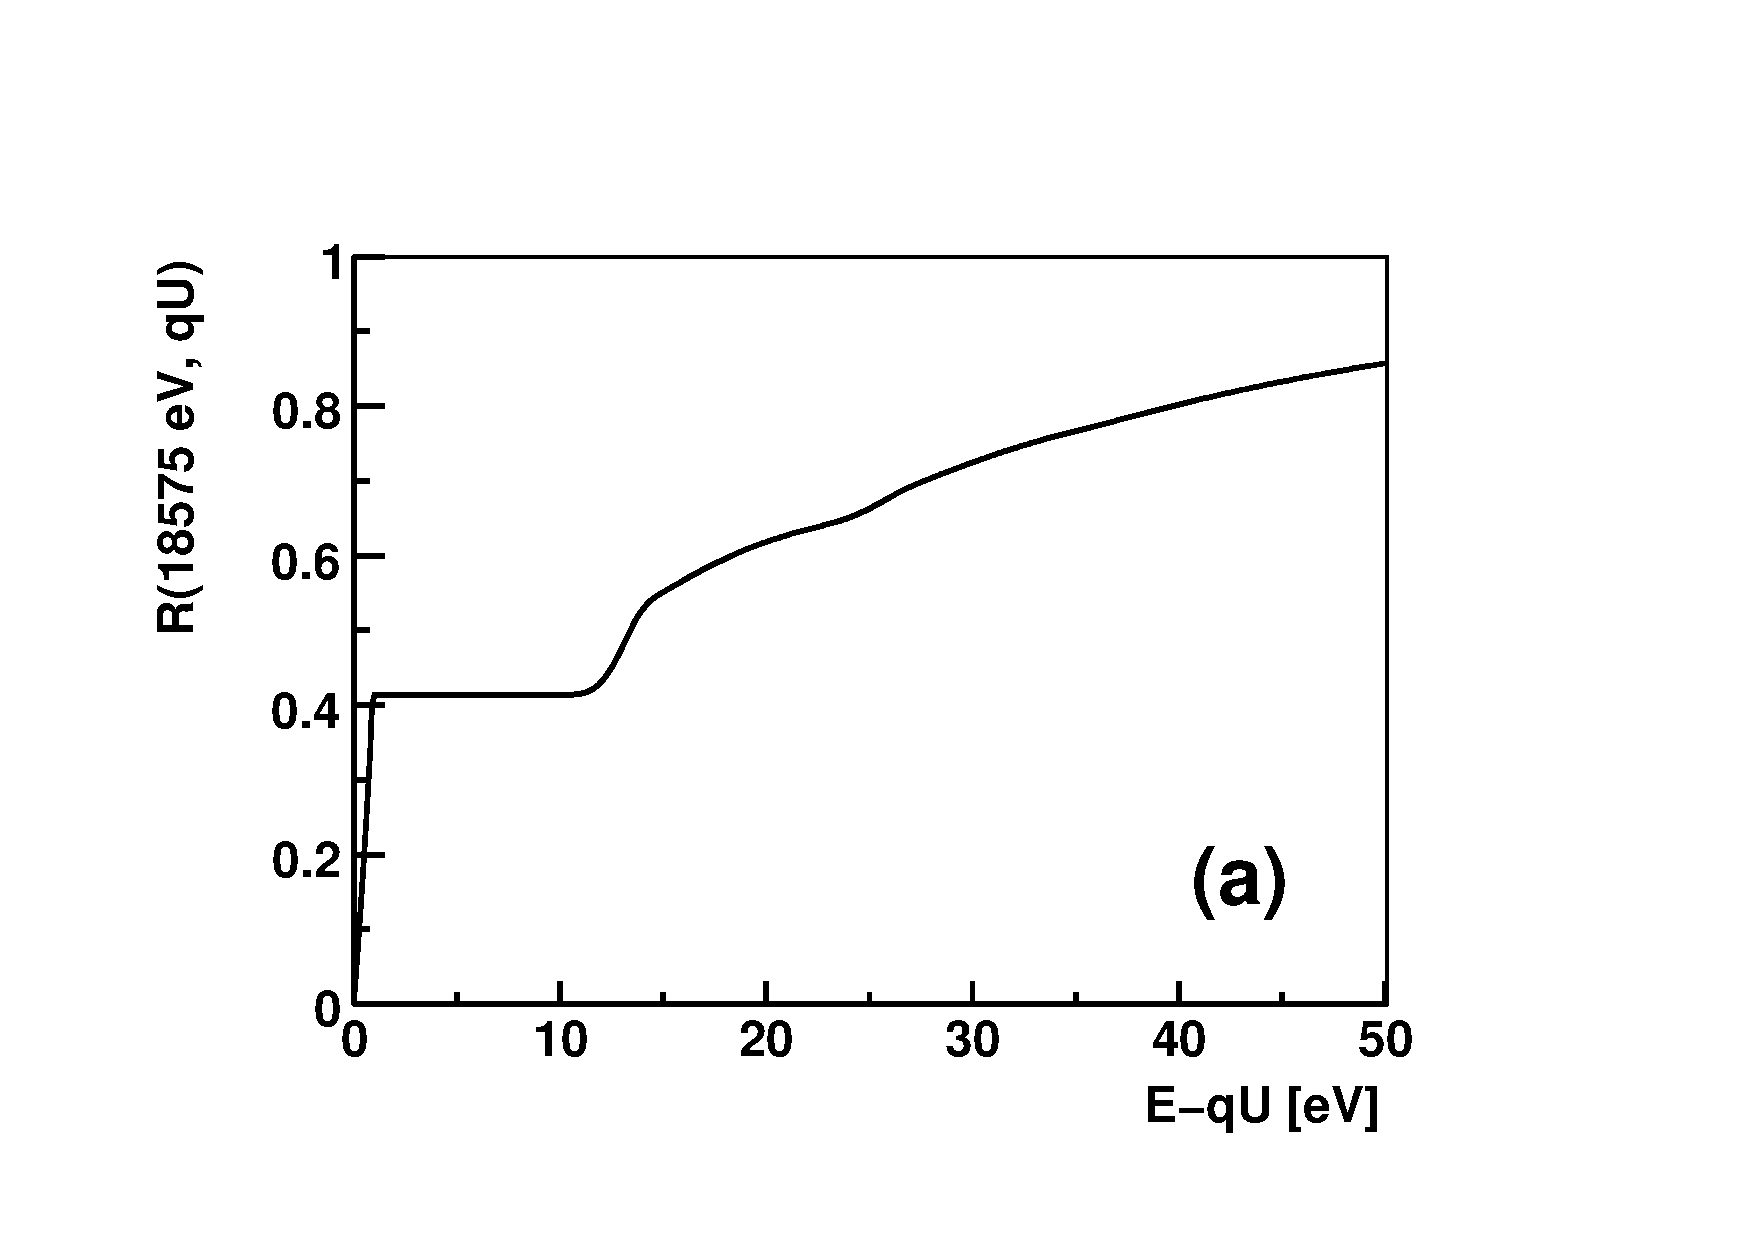
\includegraphics[width=0.50\columnwidth, trim= 40 40 40 40, clip]{images/SSCPlots/responsefunction.pdf}%
	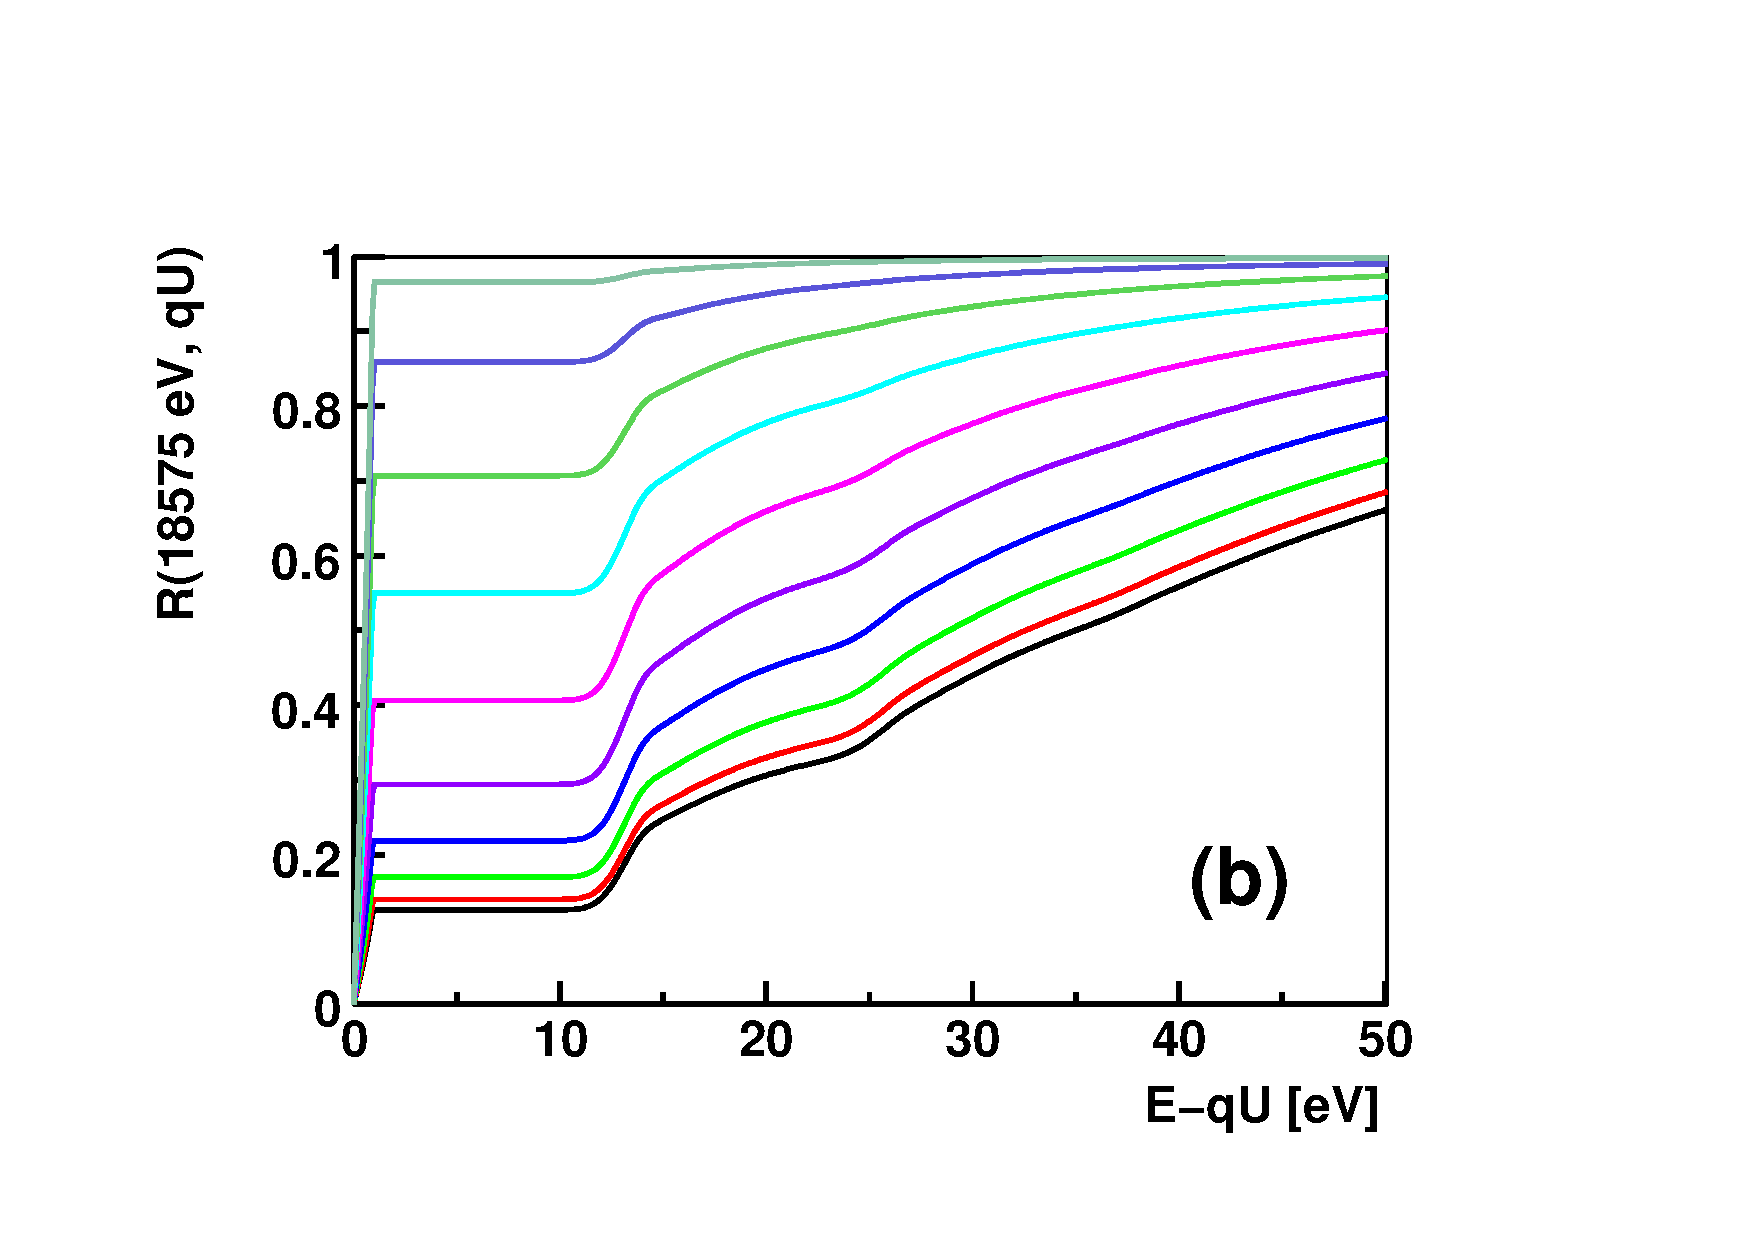
\includegraphics[width=0.50\columnwidth, trim= 40 40 40 40, clip]{images/SSCPlots/responseeverybin.pdf}%
	\caption{\textbf{(a) KATRIN standard response function $R(E,qU)$ and (b) individual response function for 10 rebinned longitudinal source pixel.}}%
	\label{fig:Response10bins}%
\end{figure}


\paragraph{Energy loss and scattering probabilities}\label{_s_s_cmain_eloss}
Inelastic scattering must be considered, since electron scattering inelastically at tritium molecules lose energy according to the energy loss function
\begin{equation}
	f(\epsilon)= \begin{cases}
	A_1 \exp\left(-\frac{2(\epsilon - \epsilon_1)^2}{\omega_1^2}\right)   & \, \epsilon < \epsilon_c \\
	A_2 \frac{\omega_2^2}{\omega_2^2 + 4 (\epsilon - \epsilon_2)^2} & \, \epsilon \geq \epsilon_c
	\end{cases}
	\label{eq:Energieverlust}
\end{equation}

with the parameters $A_1=0,204\pm0,001$, $\omega_1=1,85\pm0,02$, $A_2=0,0556\pm0,0003$, $\omega_2=12,5\pm0,1$, $\epsilon_1=12,6$, $\epsilon_2=14,30\pm0,02$ and $\epsilon_c=14,09$. The minimal energy loss for one scattering is 10 eV.

Furthermore multiple scattering is possible. To get the fraction of electrons that scatter i-\/times, the scattering probabilities P\_\-i are used: \[ P_i=\frac{1}{\rho d(1-\cos \theta_{\rm{max}})} \int_{-5m}^{+5m}dz \int_0^{\theta_{\rm{max}}} d\theta \rho(z)P_i(z,\theta)\sin\theta. \] with the column density $\rho d$, the maximal opening angle $\theta_{\rm{max}}$ and \[ P_i(z, \theta)=\exp (-\lambda \sigma_{\rm{tot}}) \frac{(\lambda \sigma_{\rm{tot}})^i}{i!} \] \[ \lambda(z, \theta) =\frac{1}{\cos \theta} \int_z^l\rho(z')dz' \] $P_i(z, \theta)$ describes the probability of an electron emitted at position z under angle $\theta$ to scatter i-\/times. $P_i(z, \theta)$ follows a Poisson distribution. $\lambda(z, \theta)$ describes the number of molecules passed by an electron during his cyclotron motion ($1/\cos{\theta}$) between emission point and spectrometer.$\backslash$ The values P\_\-i can be calculated for each part of the WGTS separately and can be used to get a specific response function. This description is more detailed than just know average values for the whole WGTS \[ P_0 = 0.413339, ~~ P_1 = 0.292658, ~~ P_2 = 0.167331, ~~ P_3 = 0.079129, ~~ P_4 = 0.031776. \]

Energy loss due to synchrotron radiation has not been considered yet, because the program uses no information on track lengths of the electrons within the magnetic fields. 
